%
% Documento: Analise e Discuss\~{a}o
%

\chapter{ANALISE E DISCUSS\~{a}O}

Os resultados obtidos nos estudos das ferramentas do BI Pentaho, foram demonstrados de forma pr\'{a}tica os conceitos de \textit{Business Intelligence} e de suas etapas estudadas no trabalho provando que as ferramentas seguem o conceito de BI. 

O Pentaho pode ser utilizado gratuitamente e posteriormente adquirir bibliotecas pagas, e ao finalizarmos a implementa\c{c}\~{a}o do BI com os dados provindos de uma planilha no formato do \textit{Microsoft Excel}, usamos na implementa\c{c}\~{a}o os conceitos de Kimball e de outros autores especialistas em BI e aplicando estes conhecimentos, obtivemos como resultados um DW com dados organizados no modelo Estrela, que proporciona a extra\c{c}\~{a}o de informa\c{c}\~{o}es \`{a} nível gerencial, criando uma triagem entre os locais que realmente necessita de um Policiamento Ostensivo e Preventivo mais eficiente, e que pode ser executado pelas for\c{c}as de seguran\c{c}a do Estado.

Este BI desenvolvido em nossa monografia serve como uma ferramenta de TI, para ajudar no planejamento e execu\c{c}\~{a}o de um determinado tipo de policiamento, pois, atuar\'{a} na preven\c{c}\~{a}o e n\~{a}o somente após a ocorrência que gera um determinado tipo penal tenha sido registrada, como \'{e} realizada atualmente. 

Este \'{e} o grande diferencial deste BI, que se utiliza dos dados providos do 181, para gerar informa\c{c}\~{o}es úteis que geram conhecimento para uma tomada de decis\~{a}o mais aprimorada.
O que seguimos neste trabalho foi simplesmente usar os recursos de coleta de dados, transforma\c{c}\~{a}o, carga, criar um local para depositar esses dados tratados e depois trabalhar estes dados de acordo com os princípios da inteligência dos negócios e necessidade do usu\'{a}rio final.

E o resultado final foi um BI com informa\c{c}\~{o}es gerenciais que possibilitam tomadas de decis\~{o}es refinadas e precisas para um melhor ajuste no policiamento em determinada regi\~{a}o, conforme Figura abaixo, abaixo, que foi elaborada com parâmetros da cidade, bairro, tipo da denúncia e os anos.

\begin{figure}[H]
	\vspace*{0,2cm}
    \centering
    \caption{Tela do \textit{Saiku} com o CUBO\_DW\_181 (cidade, bairro, tipo da denúncia e os anos)}
    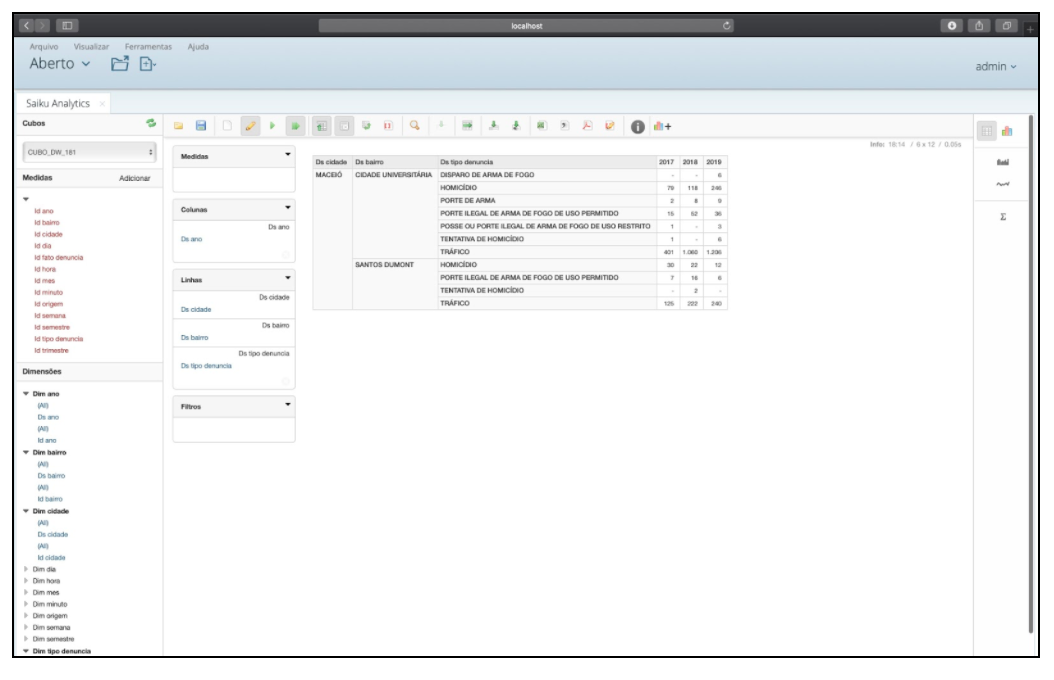
\includegraphics[width=0.6\textwidth]{./04-figuras/figura-saiku-cbta}
    \label{fig:ilustfigscbta}
\end{figure}
\vspace*{-0,9cm}
{\raggedright \fonte{Autor desta monografia, 2020.}} \\

Na figura acima, podemos ter uma compara\c{c}\~{a}o entre os anos de 2017, 2018, 2019 e 2020, de algumas denúncias em um determinado bairro e cidade, essa informa\c{c}\~{o}es podem propiciar para o gestor na \'{a}rea de seguran\c{c}a uma decis\~{a}o de aumentar ou diminuir o policiamento nestas localidades. Todas estas informa\c{c}\~{o}es usando apenas os recursos do \textit{Plugin Saiku}.

Explorando mais ainda nosso ``CUBO\_DW\_181'', podemos criar consultas com base nos dias da semana e horas, para que um refor\c{c}o na seguran\c{c}a possa se efetivada. A figura 121, demonstrar essas informa\c{c}\~{o}es e a 122, os gr\'{a}ficos de pizza com os dias da semana e os percentuais de denúncia em uma determinada hora.


\begin{figure}[H]
	\vspace*{0,2cm}
    \centering
    \caption{Tela do \textit{Saiku} com o CUBO\_DW\_181 (tipo de denúncia, semana, ano e hora)}
    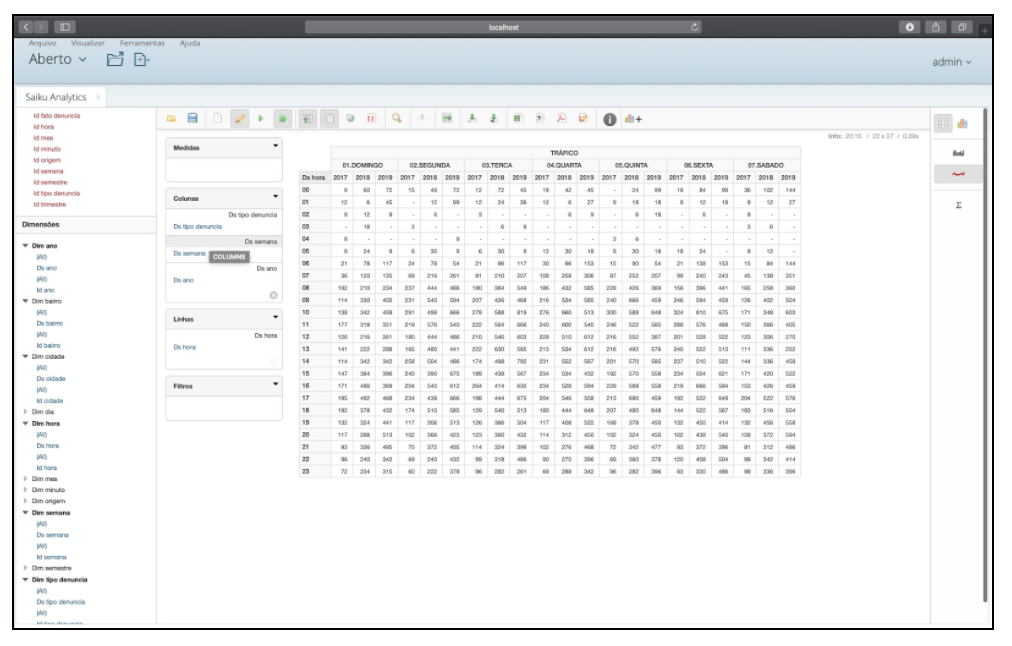
\includegraphics[width=0.6\textwidth]{./04-figuras/figura-saiku-tipo-semana-ano-hora}
    \label{fig:ilustfigstsah}
\end{figure}
\vspace*{-0,9cm}
{\raggedright \fonte{Autor desta monografia, 2020.}} \\


Com o uso deste BI, teremos muitas possibilidades de cruzamento de dados conforme o surgimentos da necessidades de informa\c{c}\~{o}es, estes últimos gr\'{a}ficos abaixo na Figura, s\~{a}o exemplos desta possibilidades.

\begin{figure}[H]
	\vspace*{0,2cm}
    \centering
    \caption{Tela do \textit{Saiku} - CUBO\_DW\_181}
    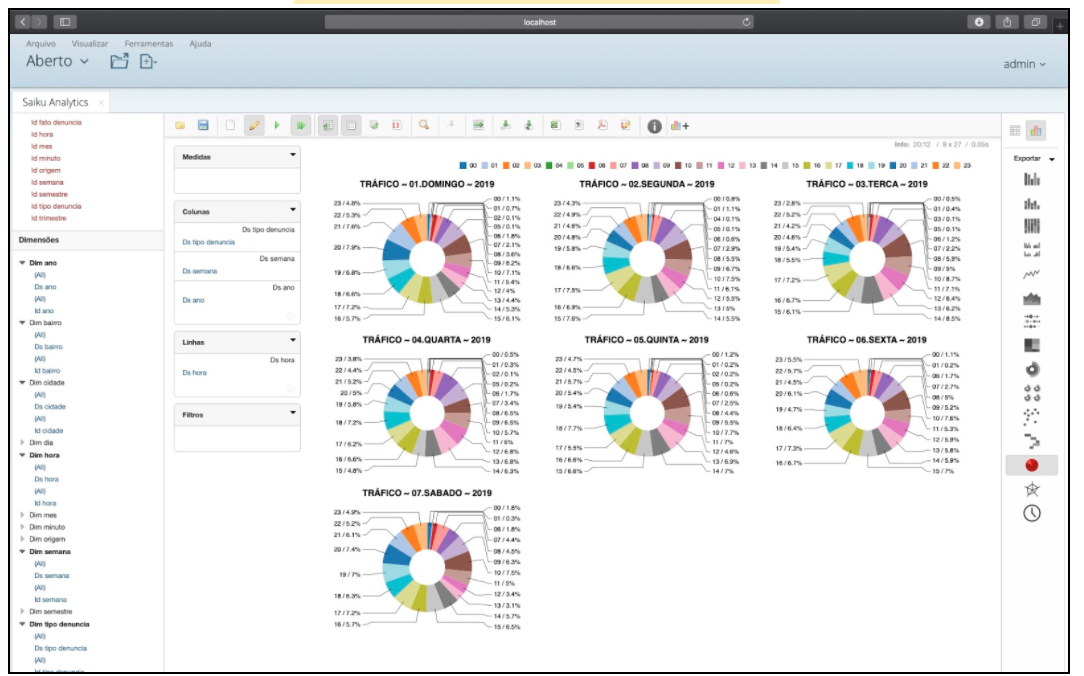
\includegraphics[width=0.6\textwidth]{./04-figuras/figura-saiku-pizza}
    \label{fig:ilustfigspizza}
\end{figure}
\vspace*{-0,9cm}
{\raggedright \fonte{Autor desta monografia, 2020.}} \\

Observado estas últimas figura percebemos que temos inúmeras possibilidades usando o ``CUBO\_DW\_181'',  criando assim os cruzamentos dos dados e gerando consultas de acordo com as necessidades de resolu\c{c}\~{a}o de problemas ligados ao excesso de denúncia em em um determinado local e espa\c{c}o de tempo.
